%================================================================
%                           N O T E S
%                           ---------
%
%                           ---------
%-----------------------------------------------------------------
%                       INTRODUCTION
%-----------------------------------------------------------------
\section{Introduction}
We now want to consider what happens inside a cylinder of different density to the outside medium. We consider our same plane wave inciding on this cylinder, see \figref{fig:problem_2}. The goal in this section is to find an expression for the velocity field over the entire domain. \par

We can divide this problem into two domains: the wave field inside the cylinder and outside the cylinder. Similar the previous problem we have
\begin{equation}
  \Phi_{tot} = \Phi_{1} + \Phi_{2} + \Phi_{in}
\end{equation}
where $\Phi_{1}$ and $\Phi_{2}$ are the potential fields for the outside and inside velocity fields respectively.

We already have an expression for the incident field from the previous chapter:
\begin{gather}
  \Phi_{in} = e^{- i(\vec{k} \cdot \vec{x})}.
\end{gather}

Physically, we still expect the wave outside the cylinder to dissipate and satisfy the Sommerfeld Radiation Condition. Hence, the solution from the previous chapter still applies, except the constant $B_n$ will be determined by the boundary condition specific for this problem. This is discussed later on in this chapter. So we have
\begin{equation}
  \Phi_1 = \sum^\infty_{n=0} \epsilon_n i^n B_2 H_n(kr) \cos(n(\theta-\alpha)).
\end{equation}

All that is left now is to find $\Phi_2$.

\begin{figure} \centering
  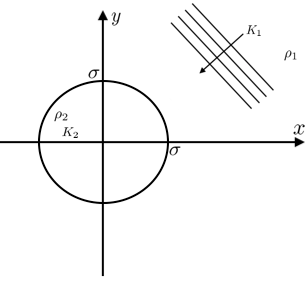
\includegraphics[width=6cm]{../figures/prob2_sketch.png}
  \caption{The transmission problem}\label{fig:problem_2}
\end{figure}

%---------------------------------------------------------------------
%
%             Potential field inside the cylinder
%
%---------------------------------------------------------------------
\section{Solution inside the cylinder}

To recover an expression for the field outside the cylinder in the previous chapter we first of all make two assumtptions: that $\Phi$ is separabale and that it satisfies the Helmholtz equation. In Proposition \ref{propn:scattered_field_differential_equations} we show that this leads to two independent differential equations, one for $\Theta(\theta)$ and one for $R(r)$. The solution for $\Theta(theta)$
\begin{equation}\label{eq:sol_inside_angular}
  \Theta(\theta) = \sum_{n=0}^{\infty} A_n \cos(n\theta) + B_n \sin(n\theta)
\end{equation}
still applies, since the only addditional assumption there is that the function must be $2 \pi$ periodic, which is clearly the case inside the cylinder too.

We are then left with the bessel differential equation to solve for $R(r)$. This problem is therefore a reformulation of the one we solved previously. Where before we had a wave that was well defined as as $r\rightarrow\infty$, we now have a wave which must be well defined as $r\rightarrow 0$.

We can make use of the propositions in \ssref{ss:limits_of_bessel_functions}, where we consider the behaviour of Bessel equations of different kind as $r\rightarrow\infty$ and $r\rightarrow 0$. Only Bessel functions of the first kind are well defined as $r\rightarrow 0$ for $n\in \bb{Z}$.

\begin{propn}
\begin{equation}
  \Phi_2 = \sum_{n=0}^{\infty} \epsilon_n i^n B_2 J_n(kr) \cos(n(\theta-\alpha))
\end{equation}
\end{propn}
\begin{proof}
  The angular component of this solution is immediate from \eqref{eq:sol_inside_angular}. The radial component of this solution is immediate from \label{eq:gen_sol_scatterin_outside_cylinder}, taking into account the different requirement on limits this solution has.
\end{proof}

We can now apply a boundary condition to find the constants we are missing.
%---------------------------------------------------------------------
%
%                 BOUNDARY CONDTION
%
%---------------------------------------------------------------------
\section{Boundary conditions}

In Chapter 1 we derived the linear wave equation from the governing equations using perturbation theory. Going back now to \ssref{ss:perturbation}, we have the modified Momentum equation \eqref{eq:perturbed_momentum}:
\begin{equation*}
  \rho \partialfrac{\vec{u}}{t} + \nabla p = 0.
\end{equation*}

We also showed in Chapter 1 that we can write $\vec{u} = \nabla \phi$, and that for $\phi = \Re[\Phi(\vec{x})T(t)]$, $T(t)=e^{-i\omega t}$, so we have
\begin{gather*}
  \frac{dT}{dt} = - i\omega T(t), \\
  \partialfrac{\vec{u}}{t} = \nabla \Re\left[\Phi \frac{dT}{dt} \right]
  = -i \omega \nabla \Re\left[ \Phi \right] = -i \omega \nabla \phi.
\end{gather*}

This means that we have a linear relationship between $\phi$, the velocity field potential and $p$, the pressure field.
\begin{align*}
  -i \omega \rho \nabla \phi &= - \nabla p \\
  \nabla (i \omega \rho \phi) &= \nabla p \\
  i \omega \rho \phi &= p \\
  p &\propto \phi
\end{align*}

Physically, we expect the pressure field to be continuous throughout the problem space, so we must also have a continuous velocity potential.
\begin{align*}
  p_1 = p_2 \Leftrightarrow \rho_1 \phi_1 = \rho_2 \phi_2
\end{align*}

Equivalently,
\begin{align*}
  \rho_1 \phi_1 &= \rho_2 \phi_2 \\
  \Leftrightarrow \rho_1 \Re[ \Phi_1 T(t) ] &= \rho_2 \Re[ \Phi_2 T(t) ] \\
  \Leftrightarrow \rho_1 \Phi_1 &= \rho_2 \Phi_2
\end{align*}
since the function $T$ does not vary with position, so it will remain the same inside and outside the cylinder. It is useful consider the derivatives of $\Phi$
instead,
\begin{align*}
  \rho_1 \Phi_1 &= \rho_2 \Phi_2 \\
  \Leftrightarrow \rho_1 \partialfrac{\Phi_1}{n} &= \rho_2 \partialfrac{\Phi_2}{n}.
\end{align*}

Where the notation $\partial / \partial n $ is shorthand for $ \nabla \cdot \vec{n},$ for $\vec{n}$ is the normal to the boundary. In particular, we're interested in what happens at the walls of the cylinder, the boundary $r=\sigma$. The normal in polar coordinates $(r, \theta)$ is $\vec{n} = (1, 0)$, hence we have
\begin{equation}
  \left.\rho_1 \partialfrac{\Phi_1}{r} \right| _{r=\sigma} = \left.\rho_2 \partialfrac{\Phi_2}{r} \right| _{r=\sigma}.
\end{equation}

This is the transmission boundary condition.

\begin{propn}
  The transmission boundary condition leads to the following relationship between the two constants
  \[ \frac{B_1}{B_2} = \frac{\rho_2 J'_n(k\sigma)}{\rho_1 H'_n(k\sigma)} \]
\end{propn}
\begin{proof}
  For simplicity we compare the $n^{\text{th}}$ term of the infinite sums, instead of the sums as a whole. We have
  \begin{align*}
    \partialfrac{\Phi^n_1}{r}
    &= \epsilon_n i^n B_1 H'_n(kr) \cos(n(\theta-\alpha)), \\
    \partialfrac{\Phi^n_2}{r}
    &= \epsilon_n i^n B_1 J'_n(kr) \cos(n(\theta-\alpha)). \\
  \end{align*}
  Hence for any given $n$
  \begin{align*}
    \left.\rho_1 \partialfrac{\Phi_1}{r} \right| _{r=\sigma} &= \left.\rho_2 \partialfrac{\Phi_2}{r} \right| _{r=\sigma} \\
    \rho_1 B_1 H'_n(k\sigma) &= \rho_2 B_1 J'_n(k\sigma)\\
    \frac{B_1}{B_2} &= \frac{\rho_2 J'_n(k\sigma)}{\rho_1 H'_n(k\sigma)}
  \end{align*}
  as required.
\end{proof}

However this doesn't give us a unique solution for the constants, we need another boundary condition, for example the specific velocity at the boundary. If we can approximate this velocity as an infinite sum
\begin{equation}
  \sum^{\infty}_{n=0} \epsilon_n i^n U_{\sigma} \cos(n(\theta-\alpha))
\end{equation}
we can find unique constants $B_1$ and $B_2$ in terms of Bessel functions that satisfy the transmission boundary condition and give the correct velocity at the boundary. The Dirichlet boundary condition is a special case of this.
